\chapter{\textsc{Newton}-Verfahren}
\section{Das \textsc{Newton}-Verfahren}
\textsc{Newton}-Richtung $d^{(k)} = -f''\left(x^{(k)}\right)^{-1}\nabla f\left(x^{(k)}\right)$ \underline{nicht} so berechnen!
Sondern über Gleichungssystem!

\[-A^{-1}\nabla f\left(x^{(k)}\right)\]
\[A = f''\left(x^{(k)}\right)\]

$\rightarrow$ Das zu lösende Gleichungssystem is linear (im Gegensatz zu dem ursprünglichen
nicht-linearen von dem \textsc{Newton}-Verfahren).

$Ax = b \overset{\text{in Matlab}}{\rightsquigarrow}$ \texttt{x = A\textbackslash b} (LU-Faktorisierung)

\[d^{(k)} = -f''\left(x^{(k)}\right)^{-1}\nabla f\left(x^{(k)}\right)\]

$f''(x^{(k)})$ positiv definit
$\Rightarrow f''(x^{(k)})^{-1}$ positiv definit
$\Rightarrow d\tr f''(x^{(k)})^{-1}d > 0 \quad \forall d \in \R^n$

Eigenwerte $\lambda_1, \ldots, \lambda_n > 0$, Eigenwerte $\frac{1}{\lambda_1}, \ldots, \frac{1}{\lambda_n} > 0$

\begin{Beispiel}{Newtonschritt\\}
\[\min f(x) = \frac{1}{2}x\tr \begin{pmatrix}
4 & 0 \\
0 & 2
\end{pmatrix}x + \begin{pmatrix}
-4 \\
-2
\end{pmatrix}\tr x + 3,\quad \text{Startpunkt: }
x^{(0)} = \begin{pmatrix}
4 \\
4
\end{pmatrix}\]



\[\nabla f(x) = \begin{pmatrix}
4 & 0 \\
0 & 2
\end{pmatrix} x + \begin{pmatrix}
-4 \\
-2
\end{pmatrix}\]
\[f''(x) = \begin{pmatrix}
4 & 0 \\
0 & 2
\end{pmatrix} \rightsquigarrow f''(x)^{-1} = \begin{pmatrix}
\frac{1}{4} & 0 \\
0 & \frac{1}{2}
\end{pmatrix}\]

\begin{enumerate}
 \item Ist der Gradient schon 0?
 \item[] $\nabla f\left(x^{(0)}\right) = \begin{pmatrix}
4 & 0 \\
0 & 2
\end{pmatrix}\begin{pmatrix}
4 \\
4
\end{pmatrix} + \begin{pmatrix}
-4 \\
-2
\end{pmatrix} = \frac{12}{6} + 0_2 \rightarrow$ nein!
 \item Berechne $d$ und $x$
 \item[] $d^{(0)} = -f''\left(x^{(0)}\right)^{-1}\nabla f\left(x^{(0)}\right) = -\begin{pmatrix}
\frac{1}{4} & 0 \\
0 & \frac{1}{2}
\end{pmatrix}\begin{pmatrix}
12 \\
6
\end{pmatrix} = -\begin{pmatrix}
3 \\
3
\end{pmatrix}$
\item[] $x^{(1)} = x^{(0)} + d^{(0)} = \begin{pmatrix}
4 \\
4
\end{pmatrix} - \begin{pmatrix}
3 \\
3
\end{pmatrix} = \begin{pmatrix}
1 \\
1
\end{pmatrix}$
  \item Gradient 0?
  \item[] $\nabla f\left(x^{(1)}\right) = \begin{pmatrix}
4 & 0 \\
0 & 2
\end{pmatrix} \begin{pmatrix}
1 \\
1
\end{pmatrix} + \begin{pmatrix}
-4 \\
-2
\end{pmatrix} = \begin{pmatrix}
0 \\
0
\end{pmatrix}$ \checkmark
\item[$\rightarrow$] \textsc{Newton}-Verfahren konvergiert nach einem Schritt für quadratische
Probleme.
\end{enumerate}
\end{Beispiel}

\textsc{Newton}-Verfahren muss gedämpft werden, weil volle Schritte teilweise
in die falsche Richtung gehen könnten (z.\,B. bei $f(x) = \sqrt{1 + x}$):
\begin{center}
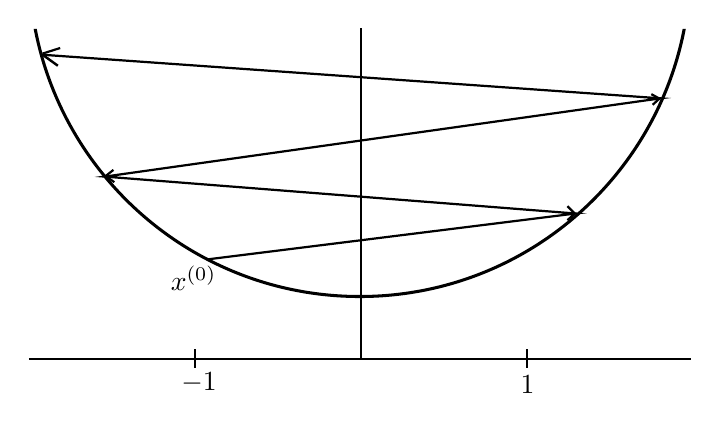
\begin{tikzpicture}[y=0.80pt, x=0.80pt, yscale=-1.000000, xscale=1.000000, inner sep=0pt, outer sep=0pt]
\begin{scope}[shift={(-0.53125,-802.625)}]
    \path[draw=black,line join=miter,line cap=butt,line width=0.832pt]
      (0.5406,951.8622) -- (299.4614,951.8622);
    \path[draw=black,line join=miter,line cap=butt,line width=0.588pt]
      (150.5199,952.1022) -- (150.5199,802.6222);
    \path[draw=black,line join=miter,line cap=butt,line width=0.965pt]
      (75.6030,947.4451) -- (75.6030,955.7591);
    \path[draw=black,line join=miter,line cap=butt,line width=0.965pt]
      (225.6030,947.4452) -- (225.6030,955.7592);
    \path[color=black,fill=black,line width=1.095pt] (2.7188,802.8438) .. controls
      (16.0212,872.0668) and (76.9019,924.3750) .. (150.0000,924.3750) .. controls
      (223.0981,924.3750) and (283.9788,872.0668) .. (297.2812,802.8438) --
      (295.8438,802.8438) .. controls (282.5683,871.3055) and (222.3498,923.0000) ..
      (150.0000,923.0000) .. controls (77.6419,923.0000) and (17.3964,871.3169) ..
      (4.1250,802.8438) -- (2.7188,802.8438) -- cycle;
    \path[draw=black,line join=miter,line cap=butt,line width=0.800pt]
      (81.3173,906.9002) -- (247.4874,886.1921) -- (34.8503,869.5246) --
      (285.8732,834.1692) -- (6.5660,814.4713);
    \path[draw=black,line join=miter,line cap=butt,line width=0.794pt]
      (6.7446,813.9662) -- (14.7009,811.4408);
    \path[draw=black,line join=miter,line cap=butt,line width=0.876pt]
      (6.6189,814.3739) -- (13.6578,819.4576);
    \path[draw=black,line join=miter,line cap=butt,line width=0.800pt]
      (282.3376,837.0734) -- (285.3681,834.2955) -- (281.7063,832.2752);
    \path[draw=black,line join=miter,line cap=butt,line width=0.800pt]
      (38.7646,866.4941) -- (35.2291,869.2720) -- (39.1434,872.0499);
    \path[draw=black,line join=miter,line cap=butt,line width=0.800pt]
      (243.8256,889.2225) -- (247.1086,886.1921) -- (243.8256,882.9091);
    \path[fill=black] (64.6498,921.0424) node[above right] (text3136) {$x^{(0)}$};
    \path[fill=black] (69.4141,967.3622) node[above right] (text3140) {$-1$};
    \path[fill=black] (222.6816,967.3622) node[above right] (text3140-7) {$1$};
\end{scope}
\end{tikzpicture}
\end{center}


\section{Das gedämpfte \textsc{Newton}-Verfahren}
\begin{enumerate}
 \item Wähle Startpunkt $x^{(0)} \in \R^n, k := 0$
 \item Ist $\nabla f(x^{(k)}) = 0_n \rightarrow$ Stop
 \item Berechne die \textsc{Newton}-Richtung $d^{(k)} = -f''(x^{(k)})^{-1}\nabla f(x^{(k)})$,
 eine effiziente Schrittweite $\sigma_k$ (z.\,B. \textsc{Armijo}) und setze $x^{(k+1)} = x^{(k)} + \sigma_kd^{(k)}$
 \item Setze $k := 1$ und gehe zu 2.
\end{enumerate}

\begin{Bemerkung}
 $d^{(k)} = -A^{-1}\nabla f(x^{(k)})$\newline
 Gradientenverfahren: $A = I_n$\newline
 \textsc{Newton}-Verfahren: $A = f''(x^{(k)})$
\end{Bemerkung}

\subsection{Konvergenz des gedämpften \textsc{Newton}-Verfahrens}
\begin{itemize}
 \item $f$ sei gleichmäßig konvex und zweimal stetig differenzierbar
 \item $\nabla f$ sei \textsc{Lipschitz}-stetig mit Konstante $L$
 \item Konvexitätsparameter $\mu$
 \item $f''(x)$ sei \textsc{Lipschitz}-stetig mit Konstante $M$, d.\,h.,
 \item[] $\norm{f''(x) - f''(y)}_F \leq M \cdot \norm{x - y}_2 \qquad \forall x, y$
 \item[] $\norm{A}_F := \sum_{i, j} |A_{ij}|^2$ (\textsc{Frobenius}-Norm)
\end{itemize}

\begin{Theorem}
 \[
 f(x^{(k)}) - f(x^*) \leq
 \begin{cases}
 f(x^{(0)}) - f(x^*) - \gamma \cdot k & \text{für } k \leq k_0\\
 \frac{2\mu^3}{M^2} \left(\frac{1}{2}\right)^{2^{k - k_0 + 1}} & \text{für } k > k_0
 \end{cases}
 \]

Seien $\delta, \beta$ die \textsc{Armijo}-Parameter, dann
$\gamma = \frac{\delta \cdot \beta^2 \cdot \eta^2 \cdot \mu}{L^2}$,
$\eta = \min \{1, 3 \cdot (1 - 2 \cdot \delta)\} \cdot \frac{\mu^2}{M}$
und $k_0$ ist die Anzahl der Iterationen bis $\norm{\nabla f(x^{(k_0 + 1)})} < \eta$.
\end{Theorem}

Gegeben sind $\gamma > 0$, $0 < \eta \leq \frac{\mu}{M^2}$. Das gedämpfte \textsc{Newton}-Verfahren konvergiert in zwei Phasen:
\begin{enumerate}
 \item Gedämpfte Phase: $\norm{\nabla f(x^{(k)})} \geq \eta$ und $f(x^{(k + 1)}) - f(x^{(k)}) \leq -\gamma$
 \item[] \textsc{Armijo}-Verfahren wählt hier typischerweise eine Schrittweite, die kleiner als $1$ ist (\glqq ge\-dämpft\grqq).
 \item Reine \textsc{Newton}-Phase: $\norm{\nabla f(x^{(k)})} < \eta$ und
 $\frac{M}{2\mu^2}\norm{\nabla f(x^{(k+1)})} \leq \left(\frac{M}{2\mu^2}\norm{\nabla f(x^{(k)})}\right)^2$
 \item[] \textsc{Armijo}-Verfahren wird sofort mit Schrittweite 1 stoppen (\glqq reine\grqq{} \textsc{Newton}-Phase).
 Sobald diese Phase erreicht ist, wird sie nicht mehr verlassen. \\
 Mit $\eta \leq \frac{\mu}{M^2}$ gilt
 $\frac{2\mu^2}{M} \cdot \left(\frac{M}{2\mu^2}\cdot\eta\right)^2 < \eta$ 
 $\Rightarrow \norm{\nabla f(x^{(k+1)})} < \eta$.
\end{enumerate}

Wir wollen $f(x^{(k)}) - f(x^*) \leq \epsilon$ erreichen. Dazu benötigt man
\[\frac{f(x^{(0)}) - f(x^*)}{\gamma} + \log\bigg(\log\bigg(\frac{\epsilon_0}{\epsilon}\bigg)\bigg)\quad\text{Iterationen.}\]

Um in die reine \textsc{Newton}-Phase zu kommen, werden höchstens $\frac{f(x^{(0)}) - f(x^*)}{\gamma}$ Iterationen benötigt.
In der reinen \textsc{Newton}-Phase ist die Konvergenzrate $\log(\log(\frac{\epsilon_0}{\epsilon}))$, mit $\epsilon_0 = \frac{2\mu^3}{M^2}$.
$\mathcal{O}(\log(\log(\frac{1}{\epsilon})))$ heißt quadratische Konvergenz (nur lokal). Zur Erinnerung: Das Gradientenverfahren hat eine lineare Konvergenz mit $\mathcal{O}(log(\frac{1}{\epsilon}))$.

Implementierungshinweise:
\begin{itemize}
 \item Gleichungssystem lösen (in GNU Octave und Matlab löst \lstinline{A\b} die Gleichung $Ax = b$) anstatt die Matrix zu invertieren.
 \item Startschrittweite $\sigma_0 = 1$ wählen.
 \item $d^{(k)} = -f''(x^{(k)})^{-1} \nabla f(x^{(k)})$ ist eine Abstiegsrichtung, wenn $H := f''(x^{(k)})$ positiv definit ist. In der Implementierung sollte daher
 $H + \gamma \cdot I_n$ mit z.\,B. $\gamma = 10^-5$ verwendet werden, was numerisch stabiler ist, da negative Eigenwerte in der \textsc{Hesse}-Matrix verhindert werden. Gggf.\,kann das Verfahren dadurch eine (oder mehr) Iterationen länger brauchen, da es nicht mehr genau das \textsc{Newton}-Verfahren ist.
\end{itemize}

\FloatBarrier
\subsection{Vergleich des gedämpften \textsc{Newton}-Verfahrens mit dem Gradientenverfahren}
\begin{table}
 \begin{tabularx}{\textwidth}[!Htb]{lXX}
  \toprule
  & \textsc{Newton}-Verfahren & Gradientenverfahren \\
  \midrule
  Speicher & $\mathcal{O}(n^2)$ ($n\times n$ \textsc{Hesse}-Matrix) & $\mathcal{O}(n)$ ($n$-dimensionaler Gradient) \\
  Berechnungen & $\mathcal{O}(n^3)$ (lineares Gleichungssystem lösen, dicht besetzt) & $\mathcal{O}(n)$ (skalieren \& addieren von $n$-dimensionalen Vektoren) \\
  \textsc{Armijo}-Verfahren & $\mathcal{O}(n)$ & $\mathcal{O}(n)$ \\
  Konditionierung & unabhängig von Kondition (zumindest Lokal) & kann stark beeinträchtigen \\
  Stabilität & \glqq etwas anfälliger\grqq & robust \\
  \bottomrule
 \end{tabularx}
 \caption{Vergleich zwischen \textsc{Newton}-Verfahren \& Gradientenverfahren}
\end{table}

Ziel ist es, den Aufwand aus den Berechnungen der \textsc{Hesse}-Matrizen zu reduzieren.

\begin{Satz}
 Sei $A$ eine reelle $n \times n$ Matrix, symmetrisch und positiv definit. Dann wird durch
 \[<x, y>_A = x\tr Ay \qquad \forall x, y \in \R^n\]
 ein Skalarprodukt definiert, und durch
 \[\norm{x}_A = \sqrt{<x,x>_A} = \sqrt{x\tr Ax} \qquad \forall x \in \R^n\]
 eine Norm auf $\R^n$ definiert. Ungleichung von \textsc{Cauchy}-\textsc{Schwarz}: $<x,y>_A \leq \norm{x}_A \cdot \norm{y}_A$.
\end{Satz}

Wir betrachten folgendes Problem:

\begin{equation}
 \begin{aligned}
  \min_{d \in \R^n} & \qquad & \nabla f(x)\tr d\\
  \text{s.\,t.}     & \qquad & \norm{d}_A = 1
  \end{aligned}
  \label{equation_20170608_1}
\end{equation}

\begin{Lemma}
 Sei $f: \R^n \rightarrow \R$ differenzierbar in $x$ mit $\nabla f(x) \neq 0_n$, und $A$ eine symmetrische, positiv definite $n \times n$-Matrix.
 Dann ist
 \[\overline{d} = -\frac{A^{-1} \nabla f(x)}{\norm{A^{-1} \nabla f(x)}_A}\]
 Lösung von \autoref{equation_20170608_1}.
 \label{lemma_20170608_1}
\end{Lemma}

\begin{proof}
 Für $d \in \R^n$ gilt
 
 \begin{equation}
  \begin{aligned}
   \nabla f(x)\tr d &= \nabla f(x)\tr \underbrace{A^{-1}A}_{=I} d = <A^{-1}\nabla f(x), Ad>\\
   &= <A^{-1} \nabla f(x), d>_A\\
   &\overset{\text{\textsc{Cauchy}-\textsc{Schwarz}}}{\geq} -\norm{A^{-1} \nabla f(x)}_A \cdot \norm{d}_A
  \end{aligned}
 \end{equation}

 Daher gilt für $\norm{d}_A = 1$: $\nabla f(x)\tr d \geq -\norm{A^{-1} \nabla f(x)}_A$.
 
 Speziell für $\overline{d}$ gilt: $\nabla f(x)\tr d = \ldots = -\norm{A^{-1} \nabla f(x)}_A$.
\end{proof}

\textsc{Newton}-Verfahren: Setze $A=f''(x)$. Im Gegensatz zum Gradientenverfahren wird in jeder Iteration eine andere Norm
(Metrik) zur Bestimmung des steilsten Abstiegs verwendet. Das gedämpfte \textsc{Newton}-Verfahren zählt daher zur Klasse der
\emph{Variable-Metrik-Verfahren}

\section{Das Quasi-\textsc{Newton}-Verfahren}
Quasi-\textsc{Newton}-Verfahren nutzen Suchrichtungen vom Typ
\[d^{(k)} = -(A^{(k)})^{-1} \nabla f(x^{(k)})\]
Diese Richtungen sind Abstiegsrichtungen wenn $A^{(k)}$ positiv definit ist.
Laut \autoref{lemma_20170608_1} sind dies die Richtungen des steilsten Abstiegs bezüglich der durch $A^{(k)}$ definierten Norm.
Verfahren, die eine solche Suchrichtung verwenden heißen Variable-Metrik-Verfahren.
Wir wollen die Schwierigkeit umgehen, $f''(x)$ zu berechnen und trotzdem noch \glqq schnell\grqq{} konvergieren.
Dazu konstruieren wir ausgehend von einer beliebigen symmetrischen, positiv definiten Matrix $A^{(0)}$ eine Folge $\{A^{(k)}\}$
symmetrischer, positiv definiter Matrizen mit den folgenden Eigenschaften:
\begin{enumerate}
 \item $A^{(k)}$ soll eine Approximation von $f''(x)$ sein.
 \item Der Übergang $A^{(k)} \rightarrow A^{(k+1)}$ soll möglichst einfach sein.
\end{enumerate}

Als Ausgangspunkt dient das Newton-Verfahren hier gilt:
\[A^{(k)}=f''(x^{(k)})\]
\[\Rightarrow\nabla f_{k+1}(x^{(k)})=\nabla f(x^{(k+1)})+A^{(k+1)}\cdot (x^{(k)}-x^{(k+1)})\overset{Taylor}{\approx}\nabla f(x^{(k)})\tag{*}\]
Also wählen wir $A^{(k+1)}$ so, dass:
\[\nabla f_{k+1}(x^{(k)})=\nabla f(x^{(k)})\]
\begin{equation}
\overset{*}{\Rightarrow}A^{(k+1)}\cdot (x^{(k+1)}-x^{(k)}) = \nabla f(x^{(k+1)})-\nabla f(x^{(k)})
\end{equation}
die sogenannte \textbf{Quasi-Newton-Gleichung}.\\

\section{Das BFGS-Verfahren}
In der Praxis hat sich die BFGS-Updateformel für $A^{(k)}$ am besten bewährt,
welche unabhängig von Broyden, Fletcher, Goldfarb und Shanno
entwickelt wurde. \\

\textbf{Herleitung der BFGS-Updateformel:} Sei
\[s^{(k)}=x^{(k+1)}-x^{(k)},\ y^{(k)}=\nabla f(x^{(k+1)}) - \nabla f(x^{(k)})\]
Start mit$A^{(0)}$ symmetrisch, positiv definit (bspw. $A^{(0)}=I_n$).\\ 
Zuerst berechnet man:
\[\tilde{A}^{(k)} = A^{(k)}-\frac{\overbrace{A^{(k)}s^{(k)}\cdot (A^{(k)}s^{(k)})^T}^{dyadisches\ Produkt}}{(s^{(k)})^TA^{(k)}s^{(k)}}\]
Dann gilt:
\[\tilde{A}^{(k)}s^{(k)} = A^{(k)}s^{(k)} - \frac{A^{(k)}s^{(k)}\cdot \cancel{s^{(k)}(A^{(k)}s^{(k)})^T}}{\cancel{(s^{(k)})^TA^{(k)}s^{(k)}}} = A^{(k)}s^{(k)} - A^{(k)}s^{(k)} = 0\]
Falls $A^{(k)}$ symmetrisch und positiv definit ist, ist $\tilde{A}^{(k)}$ symmetrisch und positiv semidefinit. Die Matrix $\tilde{A}^{(k)} - A^{(k)}$ ist symmetrisch und
\[\text{Rang}(A^{(k)}s^{(k)}\cdot (A^{(k)}s^{(k)})^T) = 1\]
da der Rang des dyadischen Produktes stets 1 ist. Daher der Name \emph{symmetrische Rang-1-Modifikation}. Danach erfolgt eine zweite symmetrische Rang-1-Modifikation mit:
\[A^{(k+1)} = \tilde{A}^{(k)}+\gamma_k\cdot w^{(k)}\cdot (w^{(k)})^T\text{ mit }\gamma_k\in\mathbb{R},\ w^{(k)}\in\mathbb{R}^n\]
Ziel: $A^{(k+1)}$ soll positiv definit sein und die Quasi-Newton-Gleichung erfüllen:
\[A^{(k+1)}s^{(k)} = y^{(k)}\]
Es muss wegen $\tilde{A}^{(k)}s^{(k)} =0$ gelten:
\[A^{(k+1)}s^{(k)} = \gamma_k\cdot w^{(k)}\cdot (w^{(k)})^T\cdot s^{(k)} = y^{(k)}\]
Wir wählen dazu:
\[w^{(k)} = y^{(k)},\ \gamma_k=\frac{1}{(y^{(k)})^Ts^{(k)}}\]
Damit $A^{(k+1)}$ positiv definit ist, muss für die Richtung $s^{(k)}$ gelten: ($\rightsquigarrow$bleibt als Voraussetzung)
\begin{equation}
(s^{(k)})^T A^{(k+1)} s^{(k)} = (y^{(k)})^Ts^{(k)} > 0
\end{equation}

\begin{Beispiel}{Voraussetzung bei quadratischen Problemen\\}
Sei $f$ eine quadratische Funktion, $Q$ positiv definit, also $f(x)=\frac{1}{2}x^TQx+q^Tx+c$
\begin{align*}
(y^{(k)})^Ts^{(k)} = (\nabla f(x^{(k+1)}) - \nabla f(x^{(k)}))^T(x^{(k+1)} - x^{(k)})\\
= (Qx^{(k+1)}+q - Qx^{(k)}-q)^T(x^{(k+1)} - x^{(k)})\\
=(x^{(k+1)} - x^{(k)})^TQ(x^{(k+1)} - x^{(k)}) \overset{Q\text{ pos. def.}}{>}0
\end{align*}
\end{Beispiel}

Das heißt obige Bedingung ist bei allen quadratischen Funktion erfüllt. Allgemeiner gilt dies auch für jede gleichmäßig konvex Funktion. (ohne Beweis)\\
Variable-Metrik-Verfahren, bei denen in jedem Iterationsschritt die
Quasi-Newton-Gleichung erfüllt ist, heißen \emph{Quasi-Newton-Verfahren}.\\
Ist $f$ zweimal stetig differenzierbar, so folgt:
\[A^{(k+1)}\cdot (x^{(k)}-x^{(k+1)}) = f''(x^{(k)} +\theta (x^{(k+1)}-x^{(k)}))\cdot (x^{(k+1)}-x^{(k)}) \] mit $0<\theta < 1$, d. h., in Richtung $x^{(k+1)}-x^{(k)}$ verhält sich $A^{(k+1)}$ ungefähr wie $f''(x^{(k+1)}$. Daher enthält $A^{(k+1)}$ Informationen über
die Krümmung von $f$ in $x^{(k+1)}$, die in die Berechnung der folgenden
Suchrichtung einfließen.\\

\textbf{Zusammenfassung:}
\begin{itemize}
\item Durch die Quasi-Newton-Gleichung ist  $A^{(k+1)}$ nicht eindeutig
bestimmt
\item In der Praxis hat sich die BFGS-Updateformel am besten bewährt
\item Beim BFGS-Verfahren berechnet man $A^{(k+1)}$ durch zwei symmetrische
Rang-1-Modifikationen von  $A^{(k)}$
\end{itemize}

\textbf{BFGS-Update-Formel:} (Rang-2-Modifikation)
\begin{equation}
A^{(k+1)} = \underbrace{A^{(k)}- \frac{A^{(k)}s^{(k)}\cdot (A^{(k)}s^{(k)})^T}{(s^{(k)})^TA^{(k)}s^{(k)}}}_{\text{Rang-1-Modifikation}}\underbrace{+ \frac{y^{(k)}(y^{(k)})^T}{(y^{(k)})^Ts^{(k)}}}_{\text{Rang-1-Modifikation}}
\end{equation}

\textbf{Das BFGS-Verfahren:}
\begin{itemize}
 \item Wähle Startpunkt $x^{(0)} \in \R^n, A^{(0)}$ symmetrisch, positiv definit, $k := 0$
 \item Ist $\nabla f(x^{(k)}) = 0_n \rightarrow$ Stop
 \item Berechne die Matrix $A^{(k)}$ nach dem BFGS-Update (für $k \geq 1$), die
Suchrichtung $d^{(k)}$ durch lösen des linearen Gleichungssystems
$A^{(k)} = -\nabla f(x^{(k)})$, die exakte Schrittweite (bei quadratischen Problemen):
\[\sigma_k=-\frac{(\nabla f(x^{(k)}))^Td^{(k)}}{(d^{(k)})^TQd^{(k)}}\]
oder bspw. die Armijo-Schrittweite sonst und setze $x^{(k+1)} = x^{(k)+\sigma_k}d^{(k)}$
\item Setze $k=k+1$.
\end{itemize}
